\documentclass[a4paper,11pt]{report}
\usepackage[T1]{fontenc}
\usepackage[utf8]{inputenc}
\usepackage{graphicx}
\usepackage{underscore}
\usepackage[italian]{babel}

\newcommand{\HRule}{\rule{\linewidth}{0.5mm}}


\begin{document}
\thispagestyle{empty}
\pagestyle{empty}

\begin{center}
\textsc{Universitità di Cagliari}\\[0.4cm]
\textsc{Facoltà di Scienze MM.FF.NN.}\\[5.5cm]

\textbf{{\large Tesina Corso SO1 - Parte 1, Pipes}}\\[0.6cm]
Davide Gessa (45712)\\[0.4cm]
\textit{A.A. 2011 - 2012\\[0.4cm]}

\vfill
\textit{8 Dicembre 2011\\[1.5cm]}


\end{center}

\newpage
\tableofcontents


\chapter{Struttura del programma}

\section{Suddivisione files}
Il codice del programma è stato ripartito in vari file cercando di dividere le varie 
funzionalità dei diversi "oggetti della scena":

\begin{itemize}
  \item alien.c alien.h - navicella aliena
  \item bomb.c bomb.h - bomba aliena
  \item control.c control.h - controllo delle iterazioni tra i vari oggetti e rendering della scena
  \item main.c - starter dell'applicazione
  \item missile.c missile.h - missile lanciato dall'astronave
  \item scores.c scores.h - gestione dei punteggi
  \item space_ship.c space_ship.h - navicella giocatore
  \item utility.c utility.h - funzioni varie utili per il funzionamento del programma
  \item spaceinvaders.h - definizioni globali
\end{itemize}

\section{Elenco funzioni}
\begin{itemize}
  \item alien_task() : gestione navicella aliena
  \item bomb_task() : gestione bomba aliena
  \item clear_quad() : cancella un area quadrata dello schermo
  \item control_check_collision() : controlla se c'è una collisione tra due oggetti
  \item control_task() : gestione della scena
  \item missile_task() : gestione di un missile
  \item render_string_array() : renderizza uno sprite nello schermo
  \item scores_add() : aggiungi un punteggio alla lista punteggi
  \item scores_load() : carica i punteggi da un file
  \item scores_save() : salva i punteggi in un file
  \item space_ship_task() : gestione navicella giocatore
  \item timevaldiff() : calcola la differenza tra due strutture timeval
\end{itemize}


\section{Il main}
La funzione main si preoccupa di creare le pipe necessarie, fare le fork per gli oggetti iniziali, ed avviare 
le relative funzioni di gestione.

\begin{enumerate}
  \item Creazione processo navicella
  \item Creazione dei processi degli alieni
  \item Avvio della funzione di controllo
\end{enumerate}




\chapter{Architettura del programma}

Ogni oggetto segue un funzionamento simile agli altri oggetti, e viene creato nel medesimo modo:
\begin{enumerate}
   \item Il padre fa una fork e continua la sua normale esecuzione
   \item Il figlio avvia la funzione di gestione dell'oggetto in questione; le funzioni di gestione
      hanno come nome oggetto_task(...) e come primo argomento ricevono tutte la pipe per inviare
      le posizioni.
 \end{enumerate} 

La funzione di gestione di un oggetto è così strutturata:
\begin{enumerate}
  \item Inizializza i dati iniziali e li inserisce in una struttura di tipo object_data_t
  \item Esegue un loop (dal quale esce al verificarsi di alcune condizioni) che ad ogni iterazione 
    produce le nuove informazioni dell'oggetto (ad esempio, tramite la tastiera nel caso
    della navicella del giocatore), le inserisce nella sua struttura e le invia
    al controllo tramite la pipe. Inoltre, il controllo può inviare informazioni ai vari oggetti
    per segnalare un avvenuta collisione (vedi sezione \ref{sec:comun}).
\end{enumerate}

Le informazioni di un oggetto sono memorizzate nella seguente struttura: 

\begin{verbatim}
///> Struttura contenente le informazioni relative all'oggetto
typedef struct
{
	int 			x;			///< Posizione x dell'oggetto
	int				y;			///< Posizione y dell'oggetto
	int 			size;		///< Dimensione dell'oggetto (sia x che y)
	
	object_type_t	type;		///< Tipo di oggetto
	int				life;		///< Vita rimanente all'oggetto
	
	pid_t			pid;		///< Pid dell'oggetto
	int				pipes[2];	///< Pipe che hanno i marzianetti per le collisioni
} object_data_t;
\end{verbatim}


\section{Comunicazione dei Task} \label{sec:comun}
Per quanto riguarda la comunicazione tra il task di controllo e gli oggetti, ho strutturato il software 
in modo che ci fosse il minor numero di Pipes, per diminuire 
l'occupazione di memoria, ed il numero di read/write; tutti gli oggetti della scena
condividono la stessa Pipe che utilizzano per inviare i propri dati al controllo (la pipe è aperta in 
scrittura lato oggetto, ed in lettura lato controllo).

Inoltre, ogni alieno ha un altra Pipe, condivisa con il controllo; la pipe è aperta in scrittura lato 
controllo, ed aperta in lettura lato alieno: viene utilizzata dal controllo per inviare lo stato
delle collisioni dell'alieno; il numero di pipe utilizzate è quindi pari a (NUMERO_ALIENI + 1).

Per gli altri oggetti, avendo la necessità di segnalare un avvenuta collisione, ho utilizzato il
meccanismo dei segnali. Se un oggetto deve essere distrutto perchè è avvenuta una collisione, 
il controllo gli invia un segnale SIGNQUIT; ogni oggetto ha al suo interno una funzione che 
gestisce questo segnale, e rende falsa la condizione del loop.

Una schematizzazione della comunicazione tra i task dell'applicazione è visibile in figura 2.1.

\begin{center}
\begin{figure}
\begin{center}
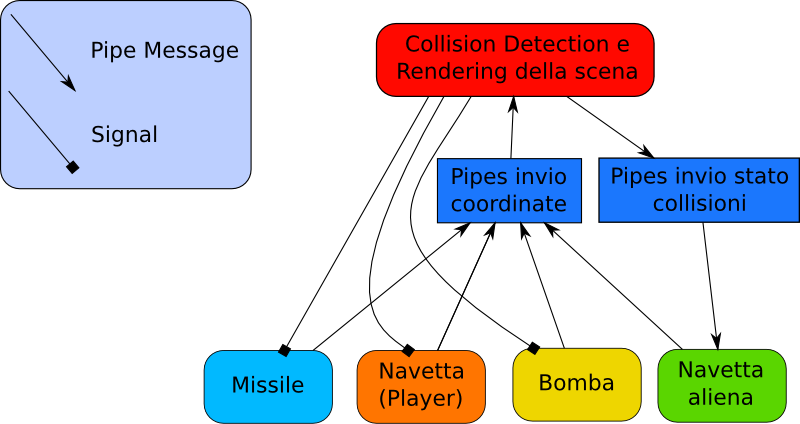
\includegraphics[scale=0.50]{comunication.png}
\end{center}
\caption{Schema di comunicazione fra i tasks}
\end{figure}
\end{center}

\section{Tasks}
Come stabilito nelle specifiche, alieni, controllo, bombe, navicella e missili utilizzano
un processo separato ciascuno.

\subsection{Controllo}
Il processo di controllo esegue un loop, ed ad ogni iterazione si occupa di:
\begin{enumerate}
  \item Ricevere dalla pipe le informazioni relative ad un oggetto
  \item Salvare in un array le informazioni ricevute
  \item Controllare se l'oggetto è in collisione con un altro oggetto, ed in tal caso, eseguire un azione appropriata
  \item Cancellare l'area di schermo occupata dall'oggetto nell'iterazione precedente
  \item Ridisegnare l'oggetto nella nuova posizione
\end{enumerate}
Il ciclo viene interrotto quando si verifica una condizione di gameover, o quando il giocatore vince.
Il processo di controllo è il padre di tutti gli oggetti della scena; quando il gioco finisce, il controllo
invia a tutti i processi ancora in vita (missili, bombe, alieni, navicella) un "messaggio" (che può essere
un opportuno messaggio nella pipe delle collisioni, per quanto riguarda gli alieni, o un segnale SIGQUIT per
tutti gli altri oggetti) per avvisare che il programma deve chiudersi.

Finito il gioco, viene aggiunto il punteggio nella lista punteggi salvata in un file, e viene visualizzata
la classifica.

\subsection{Alieno}
Si muove seguendo un percorso destra->giu->sinistra->giu come nel gioco originale;
ad ogni iterazione invia al controllo la nuova posizione, e riceve
tramite una pipe non bloccante, le informazioni relative alle collisioni:
se collide con un altro alieno, cambia direzione, altrimenti decrementa
la vita, e nel caso abbia finito le vite disponibili, si distrugge e si ricrea di livello superiore.

Ad intervalli regolari l'alieno sgancia una bomba, generando un figlio.

\subsection{Bomba}
Il processo bomba ad ogni iterazione, scende di una posizione, invia le info al controllo, e attende
un tempo predefinito; il loop termina quando riceve un segnale SIGNQUIT dal processo di controllo.

\subsection{Navicella}
Ad ogni iterazione, il processo della navicella attende un input da tastiera per comandare il movimento
o sparare dei missili; il movimento può essere solo orizzontale. 
Il lancio dei missili è limitato da un timer, che permette un certo numero di spari ogni secondo.
Premuto il tasto di sparo, la navicella crea due nuovi processi (missile destro e missile sinistro)
che avviano la funzione di gestione del missile.

\subsubsection{Missile}
Il processo missile ad ogni iterazione, sale di una posizione in verticale, si sposta di un'unità in
orizzontale (a seconda che sia un missile destro od un missile sinistro), invia le info al controllo, e attende
un tempo predefinito; come per la bomba, il loop termina quando riceve un segnale SIGNQUIT dal processo di controllo.


\section{Sincronizzazione}
Non sono state utilizzate primitive di sincronizzazione, in quanto i processi non hanno dati
condivisi. La comunicazione avviene tramite Pipes e Segnali, il kernel linux si occupa della sincronia.

\end{document}
